\documentclass[10pt,letterpaper]{article}
\usepackage[T1]{fontenc}
\usepackage{lmodern,amsmath,amssymb,mathtools,booktabs,array,graphicx,xcolor,microtype}
\usepackage[margin=.87in,top=.8in,bottom=.83in,headheight=14pt]{geometry}
\usepackage{fancyhdr,enumitem}
\usepackage[colorlinks=true,linkcolor=teal!70!black,urlcolor=teal!70!black]{hyperref}
\definecolor{teal}{HTML}{126C62}\definecolor{ink}{HTML}{193D47}
\pagestyle{fancy}\fancyhf{}\fancyhead[L]{\small\sffamily\color{ink}Intrinsic geometry of the unit oloid}
\fancyhead[R]{\small\sffamily\color{teal}Distance audit}\fancyfoot[C]{\small\thepage}
\renewcommand{\headrulewidth}{.35pt}
\newcommand{\R}{\mathbb R}\newcommand{\norm}[1]{\left\lVert#1\right\rVert}
\newcommand{\dist}{\operatorname{dist}}\newcommand{\len}{\operatorname{len}}
\newcommand{\chapterpage}{\clearpage}
\setlength{\parindent}{1.1em}\setlength{\parskip}{3pt}
\setlist{nosep,leftmargin=1.5em}
\hypersetup{pdftitle={Intrinsic distances on the unit oloid},pdfsubject={Forty-five distances, exact equations and a constructive proof}}
\begin{document}
\thispagestyle{plain}
{\small\sffamily\bfseries\color{teal} GEOMETRY \quad / \quad CONSTRUCTIVE ARITHMETIC}\par\vspace{5pt}
{\fontsize{27}{31}\selectfont\color{ink}\bfseries Intrinsic distances on the unit oloid}\par\vspace{3pt}
{\Large Forty-five verified lengths and their exact equations}\par\smallskip
\noindent All 45 distances and crossing patterns in the supplied table survive the audit. For 25 pairs the length is an elementary expression in the rational point data. For 19 more it is the value of an elementary function at the unique root of an explicit scalar equation in a rational interval. Only $P_4,P_{10}$ requires a pair of coupled equations in our description. All 45 values have rational enclosures of width $10^{-50}$. The proof allows every continuous surface path, including paths that traverse circular creases or return to them infinitely often.
\section*{The ten points}
Let $K$ be the convex hull of the closed unit disks centered at $(-1/2,0,0)$ and $(1/2,0,0)$ in the planes $z=0$ and $y=0$. Its boundary $S=\partial K$ is the oloid. In the table put $c=(1-h^2)/(1+h^2)$ and $k=2h/(1+h^2)$. The positive-quarter endpoints of a ruling are
\[
 A=(-\tfrac12-c,k,0),\qquad
 B=(\tfrac12-c/(1+c),0,\sqrt{1+2c}/(1+c)).
\]
Take $(1-s)A+sB$, then give its $y,z$ components the two indicated signs. The table retains the original exact choices. The last three columns are rounded.
\begin{center}\small\renewcommand{\arraystretch}{1.09}
\begin{tabular}{@{}ccccrrr@{}}\toprule
Point & $h$ & $s$ & signs & $x$ & $y$ & $z$\\\midrule
\csname @@input\endcsname data/point_rows.tex 
\bottomrule\end{tabular}\end{center}
\begin{center}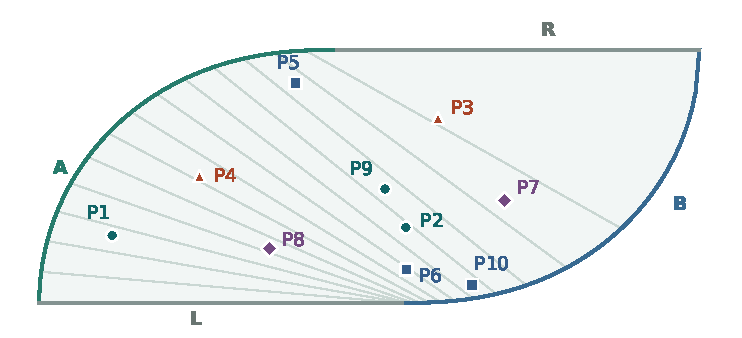
\includegraphics[width=.65\linewidth]{figures/chamber.pdf}\end{center}
\noindent\small The folded and developed points. A and B are circular arcs in space. L and R are straight rulings in symmetry planes. Pale lines connect the two ends of a ruling. The figure uses $V$ horizontally and $U$ vertically.
\normalsize

\chapterpage\section{The distance table}
The length uses the unit disk radius as its unit. A word lists successive contacts from the lower point index to the higher. A dash means both endpoints lie in one chamber and its developed chord suffices. Values here are correctly rounded to 15 places. The file \texttt{data/refined\_distances.csv} gives the enclosure endpoints and the correctly rounded 40-place values.
\begin{center}\small\renewcommand{\arraystretch}{1.18}
\begin{tabular}{@{}crl@{\hspace{2.3em}}crl@{}}\toprule
Pair & Distance & Via & Pair & Distance & Via\\\midrule
\csname @@input\endcsname data/lengths.tex 
\bottomrule\end{tabular}\end{center}
Every listed route is separated strictly from every other reduced word for its pair. There are eight direct routes, 25 with one contact and twelve with two. A point on a straight symmetry ruling can be a crossing even though the surface there is smooth.
\begin{center}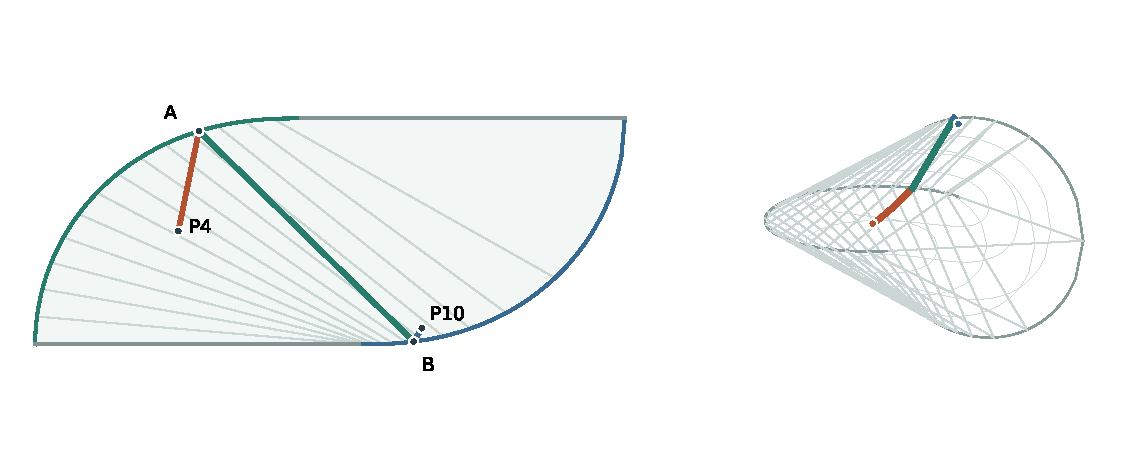
\includegraphics[width=.74\linewidth]{figures/two_creases.pdf}\end{center}
\noindent\small The $P_4$--$P_{10}$ minimizer crosses both circular arcs. Its three legs have lengths approximately $0.546382604$, $1.608380452$ and $0.083799327$. The ambient chord has length $1.742182523$.
\normalsize

\chapterpage\section{Elementary formulas for twenty-five pairs}\label{sec:elem}
Here is one lookup formula for all rows labelled with a dash, L, R, LR or RL. For a point with data $(h,s)$ put $d=1+h^2$, $z=\sqrt{3-h^2}$, and
\begin{align*}
 \alpha &=\operatorname{atan2}(hz,1-h^2)\in[0,\pi],&
 m&=\frac{2hz[2-s(3+h^2)]}{d},\\
 n&=\frac{8h^2+s(9+3h^2+2h^4)}{d},&
 (U,V)&=\frac{\sqrt3}{9}\left(2\alpha+m,\log d+n\right).
\end{align*}
The second line gives the two developed coordinates in the positive chamber. All constants in it are tabulated below. For $P_3,P_5,P_7$ the angle is in the second quadrant, and $\alpha_9=\pi/2$. In all other rows it is in the first quadrant.
\begin{center}\small\renewcommand{\arraystretch}{1.16}
\begin{tabular}{@{}rrrrr@{}}\toprule
$i$&$d_i$&$\tan\alpha_i$&$m_i$&$n_i$\\\midrule
\csname @@input\endcsname data/constants.tex 
\bottomrule\end{tabular}\end{center}
Choose $(\sigma,b)$ from the word in the distance table.
\[
\begin{array}{c|ccccc}
 \text{word} & \text{direct} & \mathrm L & \mathrm R & \mathrm{LR} & \mathrm{RL}\\\hline
 \sigma & 1 & -1 & -1 & 1 & 1\\
 b      & 0 & 0  & 1  & -1 & 1
\end{array}
\]
The exact length is
\begin{equation}
 \boxed{\displaystyle
 \frac{\sqrt3}{9}\!
 \sqrt{\left[2(\alpha_i-\sigma\alpha_j)+m_i-\sigma m_j-4\pi b\right]^2+
       \left[\log(d_i/d_j)+n_i-n_j\right]^2}.}
 \label{eq:closed}
\end{equation}
Indeed, the images of L and R lie on $U=0$ and $U=W=2\pi\sqrt3/9$. Reflecting in them in word order sends the target to $(\sigma U_j+2bW,V_j)$. The triangle inequality gives its chord length as a lower bound. The chord attains the bound if it crosses the finite sides in order. For every crossed image line $U=k$, evaluate $\lambda=(k-U_i)/(\sigma U_j+2bW-U_i)$ and $V_i+\lambda(V_j-V_i)$. The checker verifies strictly increasing $0<\lambda<1$ and strict inclusion in the vertical range of each actual side. Convexity of the developed chamber, proved below, puts every refolded leg in its copy.
\par The constants come directly from the development of Dirnböck and Stachel~\cite{ds}. In the notation of Section~\ref{sec:dev}, $\alpha=\theta+\beta$. Addition of their sines and cosines gives the indicated branch of $\operatorname{atan2}$.

\chapterpage\section{Two routes less than seven millionths apart}
For $P_6,P_9$ only the $y$ sign changes. One may cross the straight side L or the curved seam B. Let $p=(U_6,V_6)$, $q=(U_9,V_9)$, and $o=(0,\sqrt3)$. The two word minima have the elementary expressions
\[
  d_L=\norm{p-(-U_9,V_9)},\qquad d_B=\norm{p-o}+\norm{q-o}.
\]
The winning L chord meets the side strictly below $o$. The B route touches the common corner $o$ of B and L. Thus the two constrained routes can get very close even when their optimal contacts differ. Substitution into \eqref{eq:closed} gives the following standalone example:
\[
 d_L=\frac{\sqrt3}{9}\sqrt{
 \left[2\arctan(2\sqrt{23}/5)+\pi-
 \frac{428\sqrt{23}}{1521}-\frac{2\sqrt2}{9}\right]^2+
 \left[\log(13/18)+\frac{13303}{1521}-\frac{71}{9}\right]^2}.
\]
The exact separation $d_B-d_L$ lies between
\[
\begin{aligned}
&0.000006882124218519015651436570772118604632254,\\[-2pt]
&0.000006882124218519015651436570772118604632255 .
\end{aligned}
\]
To prove the B formula, parametrize its full length by $G(f)$ as in Section~\ref{sec:global}. Its corner $G(1)=o$ gives a feasible upper bound. On $[0,1-2^{-10}]$ away from the last cell, ten successive dyadic splits and the cell inequality in Section~\ref{sec:cert} exclude all minima outside $[1-2^{-10},1]$. More explicitly, the excluded left children have lower bound at least one unit of $10^{-14}$ above the rounded feasible upper bound. On the last cell, direct interval substitution in
\[
 G'(f)\cdot\left(\frac{G(f)-p}{\norm{G(f)-p}}+
                         \frac{G(f)-q}{\norm{G(f)-q}}\right)
\]
gives an upper bound below $-0.0187$. The function is strictly decreasing there, including by continuity at the endpoint. This proves unique endpoint optimality for B. The files \texttt{close\_competitor.py} and \texttt{symbolic.py} reproduce the two checks.
\begin{center}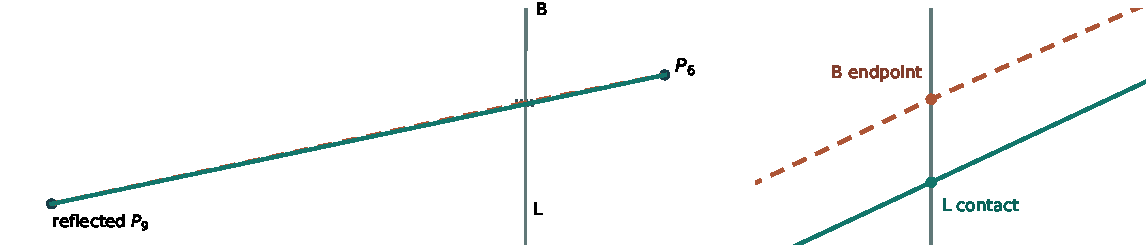
\includegraphics[width=.87\linewidth]{figures/close_pair.pdf}\end{center}
\noindent\small The target has been reflected across L. The solid line is the winning unfolded chord; the dashed line is constrained to pass through the B endpoint. The detail on the right magnifies the separation of the two contacts.\normalsize
\subsection*{What the equations determine}
The reflection formula above covers eight direct routes, fifteen straight single contacts and two straight double contacts. Of the twenty curved winners, ten cross a single curve and nine cross a curve and a straight side. A straight contact can be eliminated analytically, leaving one scalar unknown in each of these nineteen cases. The remaining word AB connects $P_4$ to $P_{10}$. Its two contact parameters cannot be selected independently. Section~\ref{sec:roots} gives the equations and isolating boxes. No assertion about the impossibility of further elementary reductions is needed.

\chapterpage\section{One quarter of the boundary}
Write $C=S\cap\{y,z\ge0\}$ and $T=2\pi/3$. In the point formulas on page 1 put $0\le t\le T$, $c=\cos t$, $k=\sin t$ and $h=\tan(t/2)$. The map $X=(1-s)A+sB$ parametrizes $C$. To see this, the vector
\[
       n=(-c,k,\sqrt{1+2c})
\]
has projection lengths $1$ and $1+c$ in the two disk planes. On each disk its unique support point is the displayed endpoint, and the two support heights are both $1+c/2$. This puts the entire segment on the boundary.
\par Conversely a point of the hull is the interpolation of one point from each disk, by grouping a convex combination. At a boundary point with $y,z>0$ both weights are positive. A supporting plane there must consequently maximize its normal on both disks at their common support height. Neither projection is zero, since a normal perpendicular to one disk strictly favors the other. Normalize the first projection to unit length and write it $(-c,k)$; the signs of the point force $k>0$ and $n_z>0$. Equality of heights forces the other projection length to be $1+c$ and $n_z^2=1+2c$. This recovers the displayed ruling. The origin is interior, as $K$ contains $\pm e_j/2$ for the three coordinate axes. Radial projection therefore identifies its boundary with a sphere, and the open quarter is dense in the closed one. Compactness of the parameter rectangle now includes its boundary. The same support argument gives injectivity. Positive interpolation weights force both endpoints to be the unique maximizing points. On each exposed circle arc the parameter is injective, the two arcs are disjoint, and positive weights cannot represent an arc endpoint using a second ruling. The polynomial inverse bounds below also give injectivity directly.
\par The result is four sign-reflected chambers. The sides with $y=0$ are B ($s=1$) and L ($t=0$). Those with $z=0$ are A ($s=0$) and R ($t=T$). The double counts at the corners are precisely the gluings from these descriptions.
\section{An elementary planar development}\label{sec:dev}
Let $v=\sin\theta=h/\sqrt3$, $w=\cos\theta$, $d=1+3v^2$ on $0\le\theta\le\pi/2$. Put $\beta=\operatorname{atan2}(2v,w)$, $\phi=2(\theta-\beta)$, $e=(\sin\phi,\cos\phi)$ and $J(u_1,u_2)=(u_2,-u_1)$. Define
\begin{align*}
 a&=\left(\tfrac{2\sqrt3}{9}(\theta+\beta+6vw/d),
             \tfrac{\sqrt3}{9}(\log d+8(1-1/d))\right),\\
 e&=\left(-2v(1+v^2)w/d,(1+v^2+2v^4)/d\right),\quad
 b=a+\sqrt3 e,\quad F(s,\theta)=a+s\sqrt3 e .
\end{align*}
We denote the same lower endpoint evaluated at circular arclength $t$ by $a[t]$. At the ends $a[0]=(0,0)$ and $a[T]=(W,K_0)$ where
$K_0=\sqrt3(6+\log4)/9$. Put $H=K_0+\sqrt3$.
The opposite endpoint is $(W,H)-a[t^*]$ with $\cos t^*=-c/(1+c)$.
Indeed the starred parameters are $v^*=w/\sqrt d$, $w^*=2v/\sqrt d$, $d^*=4/d$, $\theta^*=\pi/2-\beta$, $\beta^*=\pi/2-\theta$. Substitution proves the identity, including the endpoints.

\chapterpage\subsection*{The metric in both charts}
Primes in this section refer to $\theta$. Differentiation gives
$t'=2\sqrt3 w/d$, $\beta'=2/d$, $e'=\phi' Je$ and
\[
  a'=t'(ve+wJe),\qquad a_t=(w^3, v(3+v^2))/d .
\]
In space set $E=(B-A)/\sqrt3$, $\widehat n=n/|n|$ and $N=\widehat n\times E$.
Squaring the three component differences gives $|B-A|^2=3$. Substitution also gives
$A_t\cdot E=v$ and $A_{tt}\cdot E=\sqrt3 w^2/2$.
Both $A'$ and $B'$ are in the support plane. Thus $A_t=vE+wN$ (the sign is positive at $t=0$ and fixed on $w>0$), and $E'=\lambda N$. Differentiating $A_t\cdot E=v$ gives
\[
   \lambda=(w-t'\sqrt3 w^2/2)/w=2(3v^2-1)/d=\phi'.
\]
The frame formulas themselves extend continuously, with continuous derivatives, to both ends. Let $Q_\theta\colon\R^2\to\R^3$ take $e,Je$ to $E,N$. It is a linear isometry and $dX=Q_\theta\,dF$. In particular $Q'_\theta e=0$, by differentiating $Q_\theta e=E$. These last two identities will control lengths even at the corners where the parametrization loses rank.

\subsection*{Convexity and coverage of the development}
The tangent angle of $a$ from the $U$-axis is $2\beta-\theta$, by $a_t=ve+wJe$. Its derivative $4/d-1$ is positive on the open interval. Thus $a$ is the graph of a strictly convex increasing function $f$ on $[0,W]$, allowing a vertical tangent at $W$. The upper boundary is the graph of $g(u)=H-f(W-u)$. The chord bound $f(u)\le K_0u/W$ gives $g(u)-f(u)\ge\sqrt3$. The closed region $D$ between the graphs over $[0,W]$ is convex. All rulings belong to it.
\par For an interior ruling its line has strictly negative slope, while the two graphs increase. Its intersection with $D$ is precisely the segment from $a$ to $b$. A unit perpendicular to that line is $\nu=(e_V,-e_U)$ with nonnegative coordinates and positive $U$ component. The two endpoint curves increase in both coordinates with $\theta$, strictly in $U$ in the interior. Hence points of smaller parameter lie on one side of the line, larger parameters on the other. For $z\in D$ with $0<z_U<W$, the continuous quantity $\nu(\theta)\cdot(z-a(\theta))$ has opposite signs at the two end rulings. It vanishes at an intermediate ruling and $z$ belongs to its segment. Uniqueness follows from separation. At $U=0,W$ each side is parametrized in full. This proves that $F$ maps the rectangle homeomorphically onto $D$. We give a finite-grid implementation of inversion below.
\paragraph{A relative chord estimate through the singular corners.}
For fixed $z\in\R^2$ define the affine isometric embedding
$T_\theta(z)=A(\theta)+Q_\theta(z-a(\theta))$. On the ruling with parameter $\theta$, it sends $F$ to $X$. Its derivative for fixed $z$ is $Q'_\theta(z-a)$ since $A'=Q_\theta a'$. The vector $Q'_\theta e$ is zero. On all of the rectangle $\|Q'_\theta\|_{\rm op}\le32$. For explicit bounds, $|\phi'|\le2$, the derivative of $(-c,\sin t)$ has norm at most $4$, and $n_z=\sqrt3 w/\sqrt d$ has derivative bounded by $8$. Since $|n|\ge1$, $|\widehat n'|\le12$, $|E'|\le2$ and $|N'|\le14$. Differentiate $Q=Ee^{\mathsf T}+N(Je)^{\mathsf T}$ to obtain the stated bound.

\chapterpage
Let $p=F(s,\theta)$, $q=F(r,\eta)$ and $x=X(s,\theta)$, $y=X(r,\eta)$. For any intermediate ruling, $p,q$ are on opposite closed sides of its line. The normal component of $q-a$ therefore has magnitude at most $|q-p|$. Integrating $T'_\xi(q)$ from $\theta$ to $\eta$ gives
\begin{equation}
 \big|y-x-Q_\theta(q-p)\big|\le32|\eta-\theta|\,|q-p| .
 \label{eq:rigid}
\end{equation}
This estimate is uniform in both ruling fractions. At a singular corner the same argument applies verbatim. There is no division by the chart Jacobian.
\par In either chart, sufficiently short chords have uniformly small $|\eta-\theta|$ by uniform continuity of the inverse, or explicitly by \eqref{eq:invmod} below. Thus corresponding sufficiently short chords have length ratio arbitrarily close to one, in both directions. A continuous curve on a compact time interval admits a partition fine enough to have this property on every further subdivision. Refine any given partition by it; the triangle inequality increases chord sums under refinement. Summing \eqref{eq:rigid}, taking the supremum, then letting the relative error tend to zero proves that $X$ and $F$ give identical lengths to every continuous parameter curve, also when the length is infinite. In particular a segment in $D$ lifts to a path on $S$ of its exact Euclidean length.

\section{Reduction of all surface paths to at most two contacts}\label{sec:global}
Write $\bar p=F\circ X^{-1}(p_x,|p_y|,|p_z|)$. Absolute values contract spatial chord distances, and preserve membership in the surface by symmetry. Hence on any subinterval $I=[u,v]$ of a continuous surface path $\gamma$,
\begin{equation}
    |\overline{\gamma(u)}-\overline{\gamma(v)}|
                   \le \len(\gamma|_I).                  \label{eq:fold}
\end{equation}
Here length is the supremum of ordered Euclidean chord sums, with value $+\infty$ allowed. Define four gates in $(U,V)$ coordinates, using $0\le f\le1$:
\[
 G_A(f)=a[Tf],\quad G_B(f)=(W,H)-a[Tf],\quad
 G_L(f)=(0,\sqrt3 f),\quad G_R(f)=(W,K_0+\sqrt3 f).
\]
For a word $w=g_1\cdots g_k$, set $z_0=\bar p,z_{k+1}=\bar q$, $z_j=G_{g_j}(f_j)$ and $L_w(f)=\sum_{j=0}^k |z_{j+1}-z_j|$. The exact intrinsic distance is the smallest of the word minima for these choices:
\[
\begin{array}{c|l}
 \text{differing signs} & \text{admissible words, in crossing order}\\ \hline
 \varnothing & \text{empty}\\
 y & \mathrm B,\mathrm L\\
 z & \mathrm A,\mathrm R\\
 y,z & \mathrm{BA,BR,LA,LR,AB,AL,RB,RL}.
\end{array}
\]
A differing coordinate vanishes somewhere on the path. Select one zero for each required coordinate and order the selected times. Every selected point lies on one of the corresponding two gates. Apply \eqref{eq:fold} between consecutive times and add. This proves the lower bound even if the two zeros coincide or the path revisits its gates infinitely often. Conversely, for any feasible contacts, all their connecting segments lie in $D$. Lift each into the current sign chamber and change the indicated sign at its end. The adjacent lifts agree at the gate because that coordinate is zero. The combined surface path realizes the chord sum. Ordinary compactness gives attainment for each word. Sections~\ref{sec:arith}--\ref{sec:formal} give finite interpretations of both inequalities and constructions of the minimizing contacts for these data.

\chapterpage\section{Verification of the global bounds}\label{sec:cert}
A numerical optimizer can suggest a contact but cannot exclude a shorter path elsewhere. Here the lower bound for each word is a finite cover of its entire parameter cube. The tree for a direct word has just one leaf. For the others the root is the full interval or square. Each internal node splits its longest side halfway, with earliest-coordinate tie breaking. Subdivision neither skips a cell nor changes an endpoint.
\par To bound one cell, enclose the image of a gate interval $[l,r]$ in a tube around the segment between its endpoint centers. Linear interpolation of a vector-valued twice differentiable curve $G$ has pointwise error at most $M(f-l)(r-f)/2$ if $|G''|\le M$. This follows by integrating $G''$ against the piecewise linear kernel for the interpolation error; the integral of its absolute value is $(f-l)(r-f)/2$. Equivalently, integrate the first-order increments on the two sides of $f$. For a circular gate, the planar tangent turns through $2\beta-\theta$; its derivative with respect to $t$ is $(4/d-1)/t'=\sqrt3 w/2$. Thus the normalized gate has $|G''|\le T^2\sqrt3/2<5$, including endpoints by continuity. A straight gate has zero second derivative. A valid tube radius $r_j$ is the larger endpoint-box error plus $5(r-l)^2/8$ on a curved gate. Treat the two route endpoints as zero-length segments with their own box errors.
\par Write $[a_j,b_j]$ for the center segments and choose any vector $d_j$ of norm at most one for link $j$. Set missing end directions to zero and $v_j=d_{j-1}-d_j$. Cauchy--Schwarz, followed by collection of the coefficient of each stop, gives the lower bound
\begin{equation}
     L_w\ \ge\ \sum_j\{\min(v_j\cdot a_j,v_j\cdot b_j)-r_j|v_j|\}.
     \label{eq:tube}
\end{equation}
Indeed the minimum of a linear functional on a segment is its smaller endpoint value, and the radius costs at most $r_j|v_j|$. A zero link also obeys the inequality. The checker constructs directions from approximate witness links and rounds towards zero; it tests the squared norm bound explicitly. Upper bounds use one feasible dyadic tuple and add endpoint radii to the rounded-up norms of center differences.
\par The original subdivision trees cover 154 possible words over the 45 pairs. Including the original separate AB localization, their replay performs 4,486 leaf or containment checks. For every nondirect winner each competing word has lower bound strictly above the exhibited upper bound. Independent floating-point optimization of all the patterns agrees with the certified winners. An exact-integer check also compares all original printed words and eight-place entries against the refined table. The dyadic near-minimizers in the original CSV supply feasible witnesses; they do not in general give stationary contacts.
\paragraph{Arithmetic enclosures.}
The first evaluator rounds every operation outwards on a fixed integer scale. Integer square-root brackets, the alternating bounds for cosine and reduced arctangent, and Machin's identity $\pi=16\arctan(1/5)-4\arctan(1/239)$ enclose the coordinates. For $x\in[1,4]$ the logarithm is $2\sum_{j\ge0}y^{2j+1}/(2j+1)$ with $y=(x-1)/(x+1)$; after $n$ terms the error is at most $2y^{2n+1}/[(2n+1)(1-y^2)]$. Machin's identity follows by two tangent doublings at $1/5$, then a subtraction at $1/239$, giving slope one in the first quadrant. The arctangent bounds follow from the finite geometric series integrated on its domain. These same facts justify the second evaluator at much higher precision.

\chapterpage
\section{Isolated equations for the twenty curved routes}\label{sec:roots}
Write $p,q$ for the two developed points in $(U,V)$ order, $T=2\pi/3$
and $G(f)$ for a gate with $0\le f\le1$. A curved gate uses its own
normalized arclength, so $G_A(f)=a[Tf]$ and
$G_B(f)=(W,H)-a[Tf]$. For a straight gate $L$ or $R$ let $J$
be reflection in its entire supporting line. The following equations
specify exact values independently of a choice of optimizer.

For each winning word containing just one curved gate, take $P=p$ and $Q=q$.
If the word starts with a straight gate, replace $P$ by $Jp$.
If it ends with a straight gate, replace $Q$ by $Jq$. Write $C$ for the
curved gate in the word. There is precisely one $f$ in its interval in
Table~\ref{tab:rootboxes} satisfying
\begin{equation}
 C'(f)\cdot\left(\frac{C(f)-P}{|C(f)-P|}
             +\frac{C(f)-Q}{|C(f)-Q|}\right)=0 .
 \label{eq:scalarcurve}
\end{equation}
The distance equals $|P-C(f)|+|C(f)-Q|$.
Indeed, when a straight gate occurs, its certified minimizing contact is
interior. For the curved contact held fixed, differentiating in the
straight contact shows that its two unit directions have equal tangential
components. Equivalently, reflection puts the two legs on one straight
line. One can also see this by minimizing the sum with the contact on
the entire supporting line. The curved contact and the other endpoint
are strictly on the same side, so the segment to the reflected endpoint
meets the line in the unique unconstrained minimizer. Its distance sum
is strictly convex as a function of the line contact, so the interior
constrained minimizer is that intersection.

For $P_4,P_{10}$ put $x=G_A(f),y=G_B(g)$. The two equations are
\begin{align}
 G_A'(f)\cdot\left(\frac{x-p}{|x-p|}+\frac{x-y}{|x-y|}\right)&=0,\nonumber\\
 G_B'(g)\cdot\left(\frac{y-x}{|y-x|}+\frac{y-q}{|y-q|}\right)&=0.
 \label{eq:doublecurve}
\end{align}
There is precisely one solution in the listed box and the distance is
$|p-x|+|x-y|+|y-q|$.

\begin{table}[!ht]\centering\small
\caption{Isolating intervals in gate order. An integer $k$ denotes the
closed interval $[k,k+3]/4096$. For the scalar equation use the integer
in the curved gate's position.}\label{tab:rootboxes}
\begin{tabular}{@{}ccl@{\qquad}ccl@{}}\toprule
Pair & Word & Interval indices & Pair & Word & Interval indices\\\midrule
$1,4$ & A & 1317 & $3,10$ & RB & 1233, 3409\\
$1,7$ & AL & 834, 2515 & $4,5$ & LA & 2119, 3575\\
$1,8$ & AL & 688, 1536 & $4,6$ & AL & 2600, 3814\\
$2,4$ & A & 3123 & $4,9$ & A & 3259\\
$2,6$ & B & 4052 & $4,10$ & AB & 3015, 3521\\
$2,7$ & BR & 3871, 1561 & $5,7$ & A & 4060\\
$2,10$ & B & 3498 & $5,8$ & A & 3625\\
$3,5$ & LA & 3853, 3766 & $6,8$ & A & 4070\\
$3,6$ & RB & 1075, 4020 & $7,9$ & BR & 2839, 1172\\
$3,7$ & B & 2981 & $9,10$ & B & 3488\\\bottomrule
\end{tabular}
\end{table}

\paragraph{Why the equations isolate the global shortest paths.}
Every minimizing tuple of the winning word lies in its box. To prove this
finite assertion, \texttt{verify\_roots.py} replays the dyadic covers in
\texttt{root\_trees.json} using the same chord-tube support bounds as the
distance certificate. Each leaf is contained in the displayed box or has
a lower bound at least one unit of $10^{-14}$ above the feasible path
upper bound. There are $1{,}457$ such leaves across the twenty covers.
All boxes are interior to the admissible cubes, so a minimizing tuple
satisfies the ordinary stationarity equations. The following positive
Hessian certificate proves uniqueness on the stated box.

For a leg displacement $r=z_{j+1}-z_j$ let $r_i$ be its derivative with
respect to contact coordinate $i$, and $r_{ih}$ its mixed derivative.
The contribution to the Hessian is
\[
 \partial_{ih}|r|=
 \frac{(r\times r_i)(r\times r_h)}{|r|^3}
       +\frac{r\cdot r_{ih}}{|r|},
 \qquad (a,b)\times(c,d)=ad-bc .
\]
All mixed $r_{ih}$ with $i\ne h$ vanish. The nonzero $r_i$ and $r_{ii}$
are the signed first and second derivatives of the incident gate.
For $A$ put $v=\tan(Tf/2)/\sqrt3$, $w=\sqrt{1-v^2}$,
$d=1+3v^2$, $\tau=(w^3,v(3+v^2))/d$. With $J_0(a,b)=(-b,a)$ one has
\[
 G_A'=T\tau,\qquad G_A''=T^2(\sqrt3 w/2)J_0\tau .
\]
The derivatives of $B$ are their negatives, both straight gates have
derivative $(0,\sqrt3)$ and their second derivatives vanish.
To bound positions on an interval it suffices to enclose their two
endpoints coordinatewise because each coordinate is monotone. The
identity $v^2=(1-\cos(Tf))/(3(1+\cos(Tf)))$ encloses all derivative
terms by interval operations. On every stated box each original and
unfolded leg has length greater than $0.064$. Summing the formula
above with outward rounding gives $D^2 L\succ I/32$. In dimension two
the checker proves positivity of the first principal minor and determinant
of $D^2L-I/32$. It separately applies the same check to the one-variable
reflected expression in each mixed case on its entire curved interval.
Integrating the Hessian on the segment joining any two distinct stationary
points would give
$(\nabla L(b)-\nabla L(a))\cdot(b-a)\ge |b-a|^2/32>0$.
Thus two such points cannot exist. This argument also supplies the
quantitative estimate
\[
       0\le L(u)-L(u_*)\le 16\,|\nabla L(u)|^2
\]
for every $u$ in the original box and its minimizing contact $u_*$. It
follows by integrating the Hessian lower bound from $u$ to $u_*$ and
completing the square.


\section{A second computation of every length}
The high-precision checker evaluates the point directly as $a+s\sqrt3 e$, independently of the first evaluator's interpolation between two evaluated arcs. For a circular contact at $f$, it uses $h=\tan(\pi f/3)$, $\theta=\arctan(v/w)$ and $\beta=\arctan(2v/w)$ at the interior arguments in the certificates. For each straight-only word it evaluates the reflected chord. A second substitution of the compact elementary formula verifies all 25 intervals once more.
\par For a curved word use the rational vector $t$ in \texttt{contacts.json} and enclose $G=\nabla L_w(t)$. The vector is checked to be in its isolating box. If $x_*$ is the minimizing contact, integrate the Hessian lower bound along $[t,x_*]$. Completing the square gives
\[
  L_w(t)-16|G|^2\le L_w(x_*)\le L_w(t),\qquad
  |t-x_*|\le32|G|.
\]
For the second inequality, take the scalar product of the integrated gradient difference with $t-x_*$ and use stationarity at $x_*$. This converts the check of a short residual into a rigorous two-sided distance estimate. The maximum enclosed gradient norm is $1.23065\cdot10^{-35}$ or smaller. The Euclidean error of each supplied contact vector is below $3.94\cdot10^{-34}$.
\par The second evaluator works with integer endpoints divided by $2^{272}$. Positive division, integer square roots and outward-rounded arithmetic are used throughout. Arctangents use two half-angle reductions and 92 alternating terms. Sine and cosine on $[0,4/3]$ use 53 terms each and the first omitted terms bound their errors. The logarithm uses 182 terms and the explicit tail above. Working precision, domain checks and the residual proof suffice even if the Newton guesses were generated by an unreliable solver. Each of the 45 output intervals lies strictly inside its predecessor. Both enclosure endpoints round to the same 40-place result in every row.
\paragraph{The two-crease example.}
For $(P_4,P_{10})$ the normalized contact fractions are, to twelve places,
\[
   (f_A,f_B)=(0.736520038778,\ 0.860018475139)\quad\text{(rounded)} .
\]
They lie strictly inside both exposed arcs. The first contact is on $z=0$ while $y>0$; after changing the $z$ sign, the second is on $y=0$ while $z>0$. The rational distance interval is
\[
\begin{aligned}
[\,&2.23856238338634037167599426689899751595587563306776,\\
   &2.23856238338634037167599426689899751595587563306777\,].
\end{aligned}
\]
All seven other reduced words cost at least $2.30821106873358$. Thus replacing either crease by an infinite straight mirror throughout the development would lose a real constraint.

\paragraph{Uniqueness of the shortest path image.}
Suppose a surface path attains the least length. Its chosen zero times give equality in every folded endpoint estimate. Between them its planar image must traverse the corresponding segment monotonically, since equality in the Euclidean triangle inequality holds at every intermediate time. The unfolded chord determines all straight-only contacts uniquely, and Section~\ref{sec:roots} determines the others. Open legs lie in the interior of $D$: every one joins an interior point to another point, or joins interior points of distinct gates, and the only straight boundary segments are L and R. Hence each open leg has a unique lift in its prescribed sign chamber. Extra pauses at a contact cannot move within its finite fiber. This proves uniqueness of the path image for each of the 45 pairs, allowing changes of speed and pauses.

\paragraph{Status of the exact descriptions.}
The rational parameters in the first table and \eqref{eq:closed} specify the elementary values without any search or numerical constants. Equations \eqref{eq:scalarcurve} and \eqref{eq:doublecurve} with their rational isolating intervals specify the other twenty without minimizing over a continuum. A certified convergent evaluation of their roots in first-order arithmetic follows below.

\section{A finite interpretation in intuitionistic PRA}\label{sec:arith}
In first-order iPRA, variables range over natural numbers. Encode signed integers by differences, rationals by a signed numerator and positive denominator, finite lists by number codes, and rational comparisons by cross multiplication. A real name here consists of a particular primitive recursive (PR) approximation with an explicit error bound at every precision. A fixed program is translated into its own first-order term. A claim for every such program is a scheme in the metatheory. For paths, the numerical statements concern finite lists of approximate samples and an explicit mesh or variation bound. The usual theorem about all continuous real paths follows from the geometric proof; it has no literal second-order quantifier in iPRA.
\subsection{Explicit inverse moduli for the two charts}
The same rectangular parameter $(s,\theta)$ represents the spatial and
planar quarters, with $v=\sin\theta$, $w=\cos\theta$, $d=1+3v^2$.
Suppose $\theta\le\eta$ and put $\delta=\eta-\theta$. For arbitrary
$r,s\in[0,1]$ we claim
\begin{equation}
 |X(r,\eta)-X(s,\theta)|\ge \delta^4/2048,\qquad
 |F(r,\eta)-F(s,\theta)|\ge \delta^5/4096 .
 \label{eq:invmod}
\end{equation}
These deliberately coarse constants include the two singular corners.

Take the spatial supporting normal $n(\theta)=(-c,\sin t,\sqrt{1+2c})$.
Its projected lengths on the two circle planes are $1,1+c$, and
$|n|=\sqrt{2(1+c)}\le2$. The support deficiency of the point
$X(r,\eta)$, measured from the plane containing $X(s,\theta)$, is
\[
 \frac{1-r}{2}|A(\eta)-A(\theta)|^2
     +\frac{r(1+c)}{2}|B(\eta)-B(\theta)|^2 .
\]
Indeed a unit circle point at chord distance $b$ from its maximizer
loses $b^2/2$ in unit support height. Here $A(\xi), B(\xi)$ denote the
two spatial endpoints at parameter $\xi$. The absolute derivatives of
the two angular arclengths are respectively $2\sqrt3 w/d$ and
$2\sqrt3 v/\sqrt d$; the second follows from
$\theta^*=\pi/2-\beta$, $d^*=4/d$. They are bounded below by
$(\sqrt3/2)\cos\theta$ and $\sqrt3\sin\theta$. The integrals of either
sine or cosine on any subinterval of length $\delta$ of $[0,\pi/2]$
are at least $\delta^2/4$, since $\sin x\ge x/2$ there. Both circular
angle increments exceed or equal $\delta^2/8$, and both chord lengths
are at least $\delta^2/16$. The inequalities $1+c\ge1/2$ and $|n|\le2$
now yield the first bound.

For the plane write $e=(e_U,e_V)$ for the unit ruling direction in
$(U,V)$ coordinates. The perpendicular $\nu=(e_V,-e_U)$ has
nonnegative entries and $\nu_U\ge1/4$ from
$e_V=(1+v^2+2v^4)/d$. Both coordinates of both endpoints $a,b$
increase with $\theta$. Their $U$ derivatives are
\[
    a_U'=2\sqrt3 w^4/d^2\ge(\sqrt3/8)w^4,\qquad
    b_U'=4\sqrt3 v^4/d\ge\sqrt3 v^4 .
\]
Now take the scalar product of
$F(r,\eta)-F(s,\theta)$ with $\nu(\theta)$; the contribution of
$F(r,\theta)-F(s,\theta)$ vanishes. The remaining projection is at least
a quarter of the $U$ increment, a convex combination of the two endpoint
increments. On any interval of length $\delta$, the integrals of
$\sin^4\theta$ and $\cos^4\theta$ are each at least $\delta^5/80$,
using $\sin x\ge x/2$ again. This proves the planar inequality.
For either $Y=X,F$ we also have
\[
 \sqrt3|s-r|\le |Y(s,\theta)-Y(r,\eta)|+
                       4\delta .
\]
In fact $|Y_\theta|$ is bounded above by the greater of the two endpoint
speeds, at most $2\sqrt3<4$, by linear interpolation and the derivative
formulas for the endpoint arclengths. These polynomial bounds turn
inverse-chart evaluation into a bounded grid search. To find parameters
to prescribed tolerance choose an image tolerance small enough by
\eqref{eq:invmod}, enumerate a parameter grid fine enough by the forward
Lipschitz bounds, and use rational approximations to choose a grid image
within that tolerance. The first inequality applies to points named in
spatial coordinates and the second to planar names, including the
planar chords used in lifting paths.


\subsection*{Finding a lift with a prescribed error}
For completeness, coverage of a planar chord admits a finite version of the intermediate-line argument. Sample $a,b$ on an angular grid with spacing at most $1/N$, joining the samples on each arc by chords. These chords and the two straight ends enclose a convex polygon $D_N\subset D$. Every point of either arc is within $4/N$ of a corresponding sampled point, since both speeds are below 4. Every point of $D$ is a convex combination of the two boundary values above and below it. Thus $D$ is within $4/N$ of $D_N$. The sampled rulings divide the polygon into convex quadrilaterals with these rulings as opposite sides. They are disjoint in their interiors by the strict ordering proved in Section~\ref{sec:dev}. Every point of one quadrilateral is within $4/N$ of its earlier segment, since each of the four vertices is, and a segment enlarged by a ball is convex. Subdividing the segment fraction with mesh $1/N$ adds at most $2/N$. Consequently the planar image grid is a $10/N$ net. Degenerate endpoint cells obey the same bounds.
\par To evaluate $F^{-1}$ at a represented planar point on a chord, compute all grid residuals with error at most $1/N$ and choose the least-index smallest rational residual. Its true value is at most $12/N$. At two precisions the chosen images differ by at most the sum of these tolerances. Formula \eqref{eq:invmod} converts this into a parameter error, including at singular corners. Thus lifting the chord and interpolating signs at a specified gate both have PR names and moduli. A chord is named by its one affine parameter; its evaluable lifted path is wholly on the surface. The same residual selection in the spatial chart follows by sampling a known chart name. For input presented only by the hull, the column sweep and support-deficit estimates in the supplied oloid report~\cite{previous} give finite surface-chart coverage. Concretely one may use their fixed-$x$ monotone $y$-sweep, whose increase over a normalized parameter interval of length $l$ is at least $l^4/256$, to recover a parameter to prescribed tolerance. This dependency concerns the equivalence of presentations of $S$.
\par The estimates in \eqref{eq:rigid} work as finite partition inequalities. For a folded spatial step of length at most $\delta$, the first inverse bound makes the multiplicative lower factor in \eqref{eq:rigid} at least $1-32(2048\delta)^{1/4}$. For a lifted planar step, the multiplicative upper factor is at most $1+32(4096\delta)^{1/5}$. Given an error allowance $e\le1/2$, use respectively $\delta\le(e/32)^4/2048$ or $\delta\le(e/32)^5/4096$. The folded planar length of a short spatial step is then at most $(1+2e)$ times its spatial length. These formulas allow quantifier-free induction on finite rational chord sums. To interpret differentiation and integration in their proof, parametrize the angle by $u=\tan(\theta/2)\in[0,1]$, so $v=2u/(1+u^2)$ and $w=(1-u^2)/(1+u^2)$. All frame entries are rational functions and square roots with explicit positive lower denominators. The arc can be integrated from its rationally evaluable derivative. Bound the first and second derivatives by sum, product and reciprocal rules on these fixed expressions and telescope Taylor remainders of size $C/N^2$ over $N$ cells. This proves \eqref{eq:rigid} with an arbitrarily small rational slack, uniformly in $s,r$. The normal projection inequality is a signed order inequality from monotonicity of the two endpoint coordinates, equally valid with rational enclosure slacks. This gives a finite-remainder reading also when an endpoint is singular.

\subsection*{Extracting gates from approximate samples}
A constructive proof of the lower bound can locate near contacts without selecting an exact zero of a real path. Suppose the signed sample chain has adjacent spatial distances at most $\delta$, and each reported signed coordinate has error at most $\delta$. Round its endpoint signs with sufficient accuracy to retain the known initial and final signs of the ten points. For each differing sign choose the first change of the rationally reported sign along the list (classify zero consistently). At one of the two neighboring samples the absolute true coordinate is at most $3\delta$: even if the two reports straddle zero only because of their errors, the true signed values are at most one step apart. Order the selected indices, allowing equality.
\par On the spatial chart,
\[
 |y|=(1-s)2\sqrt3\,v/d\ge (1-s)v/2,\qquad
 |z|=s\sqrt3\,w\sqrt d/2\ge sw/2 .
\]
Small $|y|$ therefore puts either $1-s$ or $v$ within $\sqrt{6\delta}$ of zero. The first gives a near B contact by moving along the ruling. The second gives a near L contact since $\theta\le2v$ and $|F_\theta|\le4$. For $z$ use $s$ or $w$ and $\pi/2-\theta\le2w$. In either case the folded sample is within $8\sqrt{6\delta}$ of the appropriate gate union. Bounded search can choose a gate by comparing rational residuals to both sampled sides, adding a controllable enclosure slack. This avoids deciding which of two real factors is zero. Inserting the selected gate point in the two adjacent legs costs at most twice this displacement. Summed over at most two contacts, the error is at most $32\sqrt{6\delta}$ plus the evaluation slacks.
\par If a finite sampled chain has length sum $V$, these operations give a feasible word with cost at most $(1+2e)V+32\sqrt{6\delta}$ before evaluation slacks, using the spatial step size above. A path supplied with a modulus of continuity gives a sufficiently fine spatial chain. For a lower-bound test one can restrict to $V\le10$: each distance here is below 3, so any larger chord sum already proves the bound. For $m$ samples, evaluating Euclidean point names to error $\eta$ changes the sum by at most $2m\eta$; choose $\eta$ after $m$. The constructive upper bound follows by lifting finitely many planar chords, refining arbitrary partitions of these chords, and applying the planar step estimate. All finite lists, signed decisions on approximate coordinates, successive minima and meshes are PR. These estimates cover paths whose coordinates oscillate across a symmetry plane unboundedly often.

\subsection*{A primitive recursive name for each optimal contact}
In the original normalized-arclength rectangles, set $\mu=1/32$. Every link has norm $>0.064$, and all gate speeds and accelerations are bounded by 3 and 5. The two adjacent links contribute at most $2(9/0.064+5)<292$ to any diagonal Hessian entry in absolute value, and an off-diagonal entry is at most $9/0.064<141$. Hence $\mu I\preceq D^2 L\preceq512 I$. Let $B$ denote the rational box. Coordinatewise clipping is nonexpansive, so
\[
   t\longmapsto \operatorname{clip}_{B}(t-\nabla L(t)/512)
\]
has Lipschitz constant $q=1-1/16384$. Indeed the difference uses the Hessian averaged along one segment; its eigenvalues obey the same two bounds. In dimensions one and two these norm bounds also follow by clearing denominators in the positive quadratic-form test. Starting anywhere in the box, $16384(p+1)$ iterations approximate the fixed point to $2^{-p-1}$ in exact arithmetic: the diameter is below one and $(1-1/m)^m\le1/2$ for $m\ge2$. Rounding each step with vector error at most $2^{-p-16}$ adds at most $16384\cdot2^{-p-16}$. These estimates give a PR Cauchy name by finite induction, independent of an existence principle for roots.
\par The fixed point is interior: for the supplied rational seed $t$, its distance to the fixed point is at most $|\mathcal T(t)-t|/(1-q)\le32|\nabla L(t)|$, where $\mathcal T$ is the clipped map. The checked seeds have boundary clearance greater than $10^{-4}$ and this error is below $4\cdot10^{-34}$. Hence the gradient is zero there. Strong convexity bounds every other point in the box below by its stationary cost plus the quadratic growth term. Outside the box the localization trees give a strict gap above a feasible upper bound. This produces an attaining contact name and hence a named shortest curve for each of these twenty words. The other twenty-five have direct affine reflection constructions. The name of a minimizing path is thus available in addition to a name of its length.
\section{A distance algorithm using only arithmetic and square roots}
\label{sec:formal}
The Lean observer below computes the distances at every requested precision. It obtains its own approximation to the developed arcs by finite sums. The much faster certificate computation of the printed table uses elementary functions.

\paragraph{One regular gate coordinate.}
Put $u=\tan(t/2)/\sqrt3\in[0,1]$. Write $a(u)$ for the lower developed
arc with $a(0)=0$. Its velocity follows by multiplying the unit tangent
by $dt/du=2\sqrt3/(1+3u^2)$:
\[
 a(u)=\int_0^u F(v)\,dv,\qquad
 F(v)=\frac{2\sqrt3}{(1+3v^2)^2}
       \big((1-v^2)\sqrt{1-v^2},\ v(3+v^2)\big).
\]
The tangent identity proved in \texttt{ObjectIdentities.lean} gives
$\|F(v)\|=2\sqrt3/(1+3v^2)<4$.
Here $C=a(1)+(0,\sqrt3)$ is the central-reflection vector. The four
gates are $a(v)$, $C-a(v)$, $(0,v\sqrt3)$ and $a(1)+(0,v\sqrt3)$.
The ruling with $h=\tan(t/2)$ has planar endpoints $a(u)$ and $C-a(v)$,
where
\[
 u^2=h^2/3,\qquad v^2=(3-h^2)/(3(1+h^2)).
\]
For the second identity insert $c'=-c/(1+c)$ into
$v^2=(1-c')/[3(1+c')]$. The selected point is the convex
combination with weights $1-s,s$.

\paragraph{A uniform rational evaluator.}
Given precision $n$, put $N=2^{n+6}$ and $M=2^{n+12}$.
An input $q=A/B\ge0$ with $B>0$ has the lower root approximation
\[
 R_M(q)=M^{-1}\operatorname{isqrt}\!\left(\left\lfloor
                M^2 A/B\right\rfloor\right).
\]
Its error is less than $1/M$ by the two integer square inequalities.
For $i=0,\ldots,M-1$ evaluate $F(i/M)$, using $R_M(3)$ and
$R_M(1-(i/M)^2)$ for the two roots. Round each final coordinate down
to a multiple of $1/M$. Sum these vectors and divide by $M$ to form
all prefix left sums $a_M(k)$, $0\le k\le M$.
To evaluate $a(u)$ or $a(v)$ at a selected endpoint, take the mesh
index $\lfloor M u\rfloor$ or $\lfloor M v\rfloor$ by the same integer
square root. For a gate contact $i/N$, use index $iM/N$, an integer.
Use the same corner and constant for all reflections. All operations have
explicitly bounded loops.

For the error estimate, $v\mapsto v^2$ is 2-Lipschitz and
$t\mapsto t\sqrt t$ is $3/2$-Lipschitz on $[0,1]$.
For the latter factor $a^3-b^3$ and $a^2-b^2$ with
$a=\sqrt t$, $b=\sqrt{t'}$:
$a^2+ab+b^2\le 3(a+b)/2$. The equality case $a=b=0$ is immediate,
and the resulting non-strict inequality can be used without division by
$a+b$. The factor $(1+3v^2)^{-2}$ is 12-Lipschitz by the difference
of reciprocals, and $v(3+v^2)$ is 6-Lipschitz and lies in $[0,4]$.
The two coordinates of $F$ therefore have Lipschitz bounds $60$ and
$216$, giving the Euclidean bound $225$.
At a mesh node the two root replacements and coordinate roundings have
combined Euclidean error at most $16/M$, since before rounding, coordinate
errors are at most $6/M$ and $8/M$, respectively. Each full left sum
has error at most $225/(2M)+16/M$. Truncating an endpoint costs at
most $4/M$. Thus every evaluated $a$ is within $140/M$,
$C$ is within $141/M$, and every developed endpoint, gate point, or
chosen convex combination is within $300/M$ of its exact value.

For every permissible word sample all contact coordinates on the
$N$-mesh. Evaluate a chord of the approximated endpoints by $R_M$
applied to its squared norm. Take the minimum $O_n$ of these integer
costs divided by $M$. Each word has at most three legs, so each sampled
cost differs from its true cost by at most $3(600+1)/M=1803/M$.
Moving one contact changes the two incident chords by at most $8/N$.
Moving two costs at most $16/N$. Comparing every exact competitor
with its rounded competitor, and comparing the finite minimizing
witness with its own exact mesh cost, yields the asymmetric enclosure
\[
 O_n - 1803/M -16/N\ \le\ d\ \le\ O_n+1803/M .
\]
In particular $|O_n-d|<2^{-n}$. This is a uniform algorithm with a
proof of its precision in ordinary mathematics. The implementation is
in \texttt{Observer.lean}. The branch certificates serve the same 45
pairs more efficiently at the decimal precision of the tables.

\paragraph{What iPRA can express.}
Encode a signed integer by a pair of naturals, rational comparisons
by cross multiplication, rational lists by primitive recursive pairing,
and each finite candidate by its word and its two mesh indices (use
dummy indices for shorter words). A bounded scan selects the smallest
index of minimum cost. Arrays in the implementation can equivalently be
recomputed by prefix sums. These encodings use composition and primitive
recursion only. For a formula with integer quantities over a common
positive denominator, $a\le b$ is the quantifier-free equation
$a\mathbin{\dot-}b=0$ on natural numerators after moving negative
parts across the inequality. A bounded universal check is the test
that the sum of its Boolean failures vanishes. Thus the target Cauchy
theorem can be stated internally, for every $m\ge n$, as
$|O_m-O_n|\le2^{-m}+2^{-n}$ with denominators cleared.
The finite-chain formulation of the surface restriction and the moduli in Section~\ref{sec:arith} give geometric meaning to this arithmetic target.

\section{Lean verification and the remaining derivations}
The enclosed files were checked with Lean 4.32.0 and, where specified,
the ProveIt development at commit
\texttt{09fe17194da14cdd100947737952e44100bb71b8}.
\begin{itemize}
\item \texttt{SurfaceDistance.lean} checks the older metric definitions,
the contraction of spatial variation under folding, zero-coordinate hits by continuity, the lower bound for all four sign patterns conditional on the chamber estimates, and the statements
\texttt{ExactTable}, \texttt{NumericalTable}. These last two are
definitions of propositions. Their proofs are open.
\item \texttt{FiniteRoutes.lean} proves attainment of the one- and
two-index mesh search, the two-sided stability of minima under explicit
maps with error bounds, and soundness of recursive certificate coverage
at every rational parameter pair. The last theorem takes proven local
leaf bounds as hypotheses.
\item \texttt{Observer.lean} implements the above total arithmetic
observer and the ten inputs. \texttt{ReplayObserver.lean} evaluates one
example in each contact-count class. The proved error bounds above
have yet to be attached to the executable as kernel theorems.
\item \texttt{ObjectIdentities.lean} supplies five universally closed
ordinary iPRA derivations of the type
$[]\vdash_{\rm PRAAx}\varphi$: the squared ruling identity, the tangent
identity, the two-dimensional Lagrange identity behind the support bound,
the two-by-two Sylvester identity, and completion of squares for a
gradient residual. These are object-language equations over signed
pairs of arbitrary natural terms.
\item \texttt{DecimalTable.lean} uses \texttt{by decide} to check integer interval nesting, widths, 8- and 40-place rounding, pair coverage and the stated residual bounds across the concrete rows. Its inputs are the rational endpoints from the separate analytic enclosure proof.
\item \texttt{ObjectMesh.lean} derives an iPRA minimum-transfer
sequent. Let $f,g$ be coarse and fine costs in common integer units
and $j$ the fine least minimizer. If $r(j)$ is a feasible coarse index
and $f(r(j))\le g(j)+E$, then $\min f\le\min g+E$. The closed sequent
is uniform in the bounds, packed geometric input and error numerator
for each fixed choice of three primitive recursive expressions.
\end{itemize}

\paragraph{Remaining implementation steps.}
First compile the displayed rational routines to the existing
\texttt{PR}/\texttt{PTm} definitions of ordinary iPRA. Use the modules for pairing, integer division and bounded sums. The least-witness operation is provided by \texttt{ApproximateWitness}. For the Cauchy derivation,
compare two prefix sums by grouping fine cells into coarse cells.
Over a coarse block the sum of the distances to its left endpoint is
at most the number of fine cells times $1/(2M_{\rm coarse})$.
Apply the algebraic Lipschitz and square-root inequalities above
termwise. For a partial final block use the endpoint error bound.
Map fine contacts to coarse contacts by integer division and embed
coarse contacts by multiplication. Applying minimum transfer in the
two directions now gives the cleared-denominator Cauchy inequality.
This step uses quantifier-free induction on prefix sums and finite
Boolean invariants. For the sharper decimal tables, implement sound
enclosures of the chart coordinates and the oloid-specific leaf-tube
bound, then instantiate rational tree coverage at the published
certificate input. Finally prove the length equality for the chamber development
and path lifting in mathlib for the external bridge to the stated class
of continuous paths. These three interfaces distinguish the arithmetic
observer, the verified decimals, and the external geometric theorem.


\paragraph{Concrete kernel replay of the integer certificates.}
The directory \texttt{lean/IntegerReplay} contains 219 checked theorems. They replay all 154 word lower-bound trees, the 45 feasible upper bounds and the 20 additional root-isolating trees. The checker tests direction norms by integer squares, evaluates the dot-product bounds, propagates dyadic cell splits and tests upper witness lengths and containment leaves. Each theorem uses kernel reduction. The numerical inputs comprise 1,276 distinct integer balls for 1,279 labeled sample instances. The Python interval proof bounds the exact chart samples by these balls. The formal bridge from the elementary chart expressions to the balls, and from the integer inequalities to the intrinsic distances of continuous curves, is still open. The 50-decimal enclosures additionally use the Hessian and gradient evaluations in the high-precision checker.

\begin{thebibliography}{9}\small\raggedright
\bibitem{ds} H. Dirnböck and H. Stachel, \emph{The Development of the Oloid}, Journal for Geometry and Graphics \textbf{1} (1997), 105--118. In particular, Theorems 1--3 give the ruling length and elementary development.
\url{https://www.heldermann-verlag.de/jgg/jgg01_05/jgg0113.pdf}
\bibitem{previous} Supplied reports, \emph{Shortest surface paths on the oloid} (original point set, gates and subdivision certificates) and \emph{The solid oloid in intuitionistic primitive recursive arithmetic} (hull coverage, support deficits and finite observations). The geometry used for the present computation is restated in this report.
\bibitem{ProveIt} V. Reshetnikov, \emph{ProveIt}, Logic/PrimitiveRecursiveArithmetic. Lean 4.32.0, revision \texttt{09fe17194da14cdd100947737952e44100bb71b8}. In particular see \texttt{Core.Pairing}, \texttt{Foundations.ApproximateWitness} and \texttt{Analysis.FiniteFTC}.
\url{https://github.com/VladimirReshetnikov/ProveIt/tree/09fe17194da14cdd100947737952e44100bb71b8/Logic/PrimitiveRecursiveArithmetic}
\end{thebibliography}
\end{document}
